\subsection{METRIZABLE TOPOLOGICAL GROUPS}

PROPOSITION 1. The left and right uniformities of a topological group G are metrizable if and only if G is Hausdorff and the identity element e of G has a countable fundamental system of neighbourhoods.

The condition is clearly necessary. Conversely, if it is satisfied, let \((\mathbf{V}_{n})\) be a fundamental system of neighbourhoods of e; if \(U_{n}\) denotes the set of pairs \((x, y) \in \mathbf{G} \times \mathbf{G}\) such that \(x^{-1}y \in V_{n}\) , then the \(U_{n}\) form a countable fundamental system of entourages of the left uniformity of G; since this uniformity is Hausdorff, it follows from §2, no. 4, Theorem 1 that it is metrizable. Similarly for the right uniformity of G.

A topological group G is said to be metrizable if its topology is metrizable. Proposition 1 then shows that its two uniformities are metrizable.

This result can be sharpened with the help of the following notion:

DEFINITION 1. A metric d on a group G (written multiplicatively) is said to be left-invariant (resp. right-invariant) if we have

\[
d (z x, z y) = d (x, y) \quad [ \text { resp. } d (x z, y z) = d (x, y) ]
\]

for all \(x, y, z\) in \(\mathbf{G}\) .

PROPOSITION 2. The left (resp. right) uniformity of a metrizable group G can be defined by a left-invariant (resp. right-invariant) metric on G.

Suppose that the fundamental system \((\mathbf{V}_{n})\) of neighbourhoods of e consists of symmetric neighbourhoods such that \(V_{n+1}^{3} \subset V_{n}\) for each n.~Then the corresponding entourages \(U_{n}\) of the left uniformity are symmetric

entourages such that \(\mathbf{U}_{n+1} \subset \mathbf{U}_n\) . The method used in the proof of Proposition 2 of §1, no. 4 allows us to construct, from the sequence of entourages \((\mathbf{U}_n)\) , a metric \(d\) on \(\mathbf{G}\) compatible with the left uniformity of \(\mathbf{G}\) ; and since for each \(z \in \mathbf{G}\) the mapping \((x, y) \to (zx, zy)\) leaves each of the \(\mathbf{U}_n\) invariant, the definition of \(d\) shows that it is a left-invariant metric. This method also holds for the right uniformity.

Note that, if the two uniformities of G are distinct, the metric d is not right-invariant, and hence in general \(d(x^{-1}, y^{-1}) \neq d(x, y)\) .

In particular, if G is a metrizable abelian group, its uniformity is defined by an invariant metric d; if G is written additively, we have

\[
d (x, y) = d (\mathrm{o}, y - x) = d (\mathrm{o}, x - y).
\]

We shall often write \(|x|\) (or \(||x||\) ) for \(d(0, x)\) ; we have then

\[
d (x, y) = | x - y |.
\]

The function \(|x|\) satisfies the following three conditions:

\begin{enumerate}
\def\labelenumi{\alph{enumi})}
\item
  \(|-x| = |x|\) for all \(x \in G\) .
\item
  \(|x + y| \leqslant |x| + |y|\) for all \(x \in G\) and all \(y \in G\) .
\item
  \(|x| = 0\) if and only if \(x = 0\) .
\end{enumerate}

Conversely :

PROPOSITION 3. Let G be an abelian group, written additively, and let \(x \to |x|\) be a mapping \(\mathbf{G} \to \mathbf{R}_+\) which satisfies conditions a), b) and c) above. Then the function \(d(x, y) = |x - y|\) is an invariant metric on G; the topology C which it defines on G is compatible with the group structure of G, and the uniformity defined by d is the same as the uniformity of the topological group obtained by endowing G with the topology C.

The function \(d(x, y)\) is a metric on \(G\) , for the relation \(d(x, y) = 0\) is equivalent to \(x = y\) by \(c\) ; we have \(d(x, y) = d(y, x)\) by \(a\) ; and

\[
d (x, y) = | (x - z) + (z - y) | \leqslant | x - z | + | z - y | = d (x, z) + d (z, y)
\]

by \(b\) ). Moreover, \(d\) is invariant, since \((x + z) - (y + z) = x - y\) . For each real number \(\alpha > 0\) , let \(V_{\alpha}\) be the set of all \(x \in G\) such that \(|x| < \alpha\) ; then the \(V_{\alpha}\) form a fundamental system \(\mathfrak{S}\) of neighbourhoods of \(o\) for the topology \(\mathfrak{C}\) , and since \(d\) is invariant, \(a + \mathfrak{S}\) is a fundamental system of neighbourhoods of \(a\) for the topology \(\mathfrak{C}\) , for each \(a \in G\) . By \(a\) , the \(V_{\alpha}\) are symmetric, and by \(b\) , we have \(V_{\alpha} + V_{\alpha} \subset V_{2\alpha}\) ; hence the topology \(\mathfrak{C}\) is compatible with the group structure of \(G\) (Chapter III, § 1, no. 2). The last part of the proposition follows immediately.

Conditions \(a), b)\) and \(c)\) are equivalent to \(c)\) together with the condition

\[
| x - y | \leqslant | x | + | y |.\tag{\(b^{\prime}\)}
\]

For \(a)\) and \(b)\) clearly imply \(b')\) ; conversely, taking \(x = 0\) in \(b')\) and using \(c)\) , we see that \(|-y| \leqslant |y|\) ; replacing \(y\) by \(-y\) it follows that \(|-y| = |y|\) , which is \(a)\) ; replacing \(y\) by \(-y\) in \(b')\) we then get \(b)\) .

PROPOSITION 4. If G is a metrizable group, then every Hausdorff quotient group G/H of G is metrizable. If G is also complete, then G/H is complete (*).

The first part of the proposition is a consequence of the fact that the identity element of G/H has a countable fundamental system of neighbourhoods in G/H; for if \((\mathbf{V}_{n})\) is a fundamental system of neighbourhoods of e in G, then the canonical images \(\dot{V}_{n}\) of the sets \(V_{n}\) in G/H form a fundamental system of neighbourhoods of the identity element of G/H (Chapter III, § 2, no. 6, Proposition 17).

To show that G/H is complete if G is complete, it is enough, by § 2, no. 6, Proposition 9, to show that every Cauchy sequence \((\dot{x}_{n})\) (with respect to the left uniformity of G/H) is convergent. We may assume, by passing to a subsequence of \((\dot{x}_{n})\) if necessary, that for each pair of indices p, q such that \(p \geqslant n\) and \(q \geqslant n\) , we have \(\dot{x}_{p}^{-1}\dot{x}_{q} \in \dot{V}_{n}\) ; this means that for each pair of points \(y \in \dot{x}_{p}, z \in \dot{x}_{q}\) , we have \(y^{-1}z \in HV_{n} = V_{n}H\) ; and therefore, for each \(y \in \dot{x}_{p}\) , the intersection of \(\dot{x}_{q}\) and the neighbourhood \(yV_{n}\) of y is not empty. Suppose then that the sequence \((V_{n})\) has been chosen so that \(V_{n+1}^{2} \subset V_{n}\) , and define inductively a sequence \((x_{n})\) of points of G, such that \(x_{n} \in \dot{x}_{n}\) and \(x_{n+1} \in x_{n}V_{n}\) ; this is possible by what has been said. It follows then by induction that for each p \textgreater{} 0 we have \(x_{n+p} \in x_{n}V_{n}V_{n+1} \ldots V_{n+p-1} \subset x_{n}V_{n-1}\) . The sequence \((x_{n})\) is therefore a Cauchy sequence in G, so it converges to a point a; and it follows immediately that the canonical image \(\dot{a}\) of a in G/H is the limit of the sequence \((\dot{x}_{n})\) .

COROLLARY 1. Let G be a complete metrizable group, let \(G_{0}\) be a dense subgroup of G and let \(H_{0}\) be a closed normal subgroup of \(G_{0}\) . If H is the closure of \(H_{0}\) in G, the quotient group \(G_{0}/H_{0}\) has a completion isomorphic to G/H.

H is a normal subgroup of G (Chapter III, § 2, no. 3, Proposition 8) and Proposition 4 shows that G/H is complete. Also if \(\varphi\) is the canonical mapping of G onto G/H, it is clear that \(\varphi(G_0)\) is dense in G/H. The result therefore follows from Chapter III, § 2, no. 7, Proposition 21.

Let \(G, G'\) be two Hausdorff abelian topological groups, and \(\hat{G}, \hat{G}'\) their respective completions. We recall (Chapter III, § 3, no. 3, Proposition 5) that if \(u\) is a continuous homomorphism of \(G\) into \(G'\) , then \(u\) is uniformly continuous and extends uniquely to a continuous homomorphism of \(\hat{G}\) into \(\hat{G}'\) , which we shall denote by \(\hat{u}\) in the remainder

of this subsection. The diagram

\pandocbounded{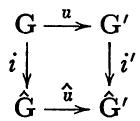
\includegraphics[keepaspectratio]{images/part001_945be03d.jpg}}

(in which \(i\) , \(i'\) are the canonical injections) is commutative. If \(v\) is a continuous homomorphism of \(\mathbf{G}'\) into a Hausdorff abelian topological group \(\mathbf{G}''\) , and if \(w = v \circ u\) , then it is follows immediately that \(\hat{w} = \hat{v} \circ \hat{u}\) .

Let H be a closed subgroup of G and let E = G/H. Let \(j: H \to G\) and \(p: G \to E\) be the canonical mappings. Let \(\overline{H}\) be the closure of H in \(\hat{G}\) ; \(\overline{H}\) is a complete group and we identify it with the completion \(\hat{H}\) of H. The continuous extension \(\hat{j}\) of j to \(\hat{H}\) is evidently the canonical injection of \(\hat{H}\) in \(\hat{G}\) .

Suppose from now on that G is metrizable. Then the canonical mapping of E = G/H into \(\hat{G}/\hat{H}\) is a topological isomorphism of E onto a dense subgroup of the complete group \(\hat{G}/\hat{H}\) (Corollary 1), and thus we may identify \(\hat{G}/\hat{H}\) with \(\hat{E}\) and the continuous extension \(\hat{p}\) of p to \(\hat{G}\) with the canonical mapping of \(\hat{G}\) onto \(\hat{G}/\hat{H}\) .

COROLLARY 2. Let G, G' be two metrizable abelian topological groups; let u: G → G' be a strict morphism with kernel N and image P. Then \(\hat{u} : \hat{G} \rightarrow \hat{G}'\) is a strict morphism with kernel \(\hat{N}\) and image \(\hat{P}\) .

Let \(u = j \circ v \circ p\) be the canonical factorization of \(u\) , where \(v\) is an isomorphism of the topological group \(G/N\) onto the topological group \(u(G) = P\) . We have \(\hat{u} = \hat{j} \circ \hat{v} \circ \hat{p}\) , and we have seen that \(\hat{p}\) is the canonical mapping of \(\hat{G}\) onto \(\hat{G}/\hat{N}\) , and that \(\hat{j}\) is the canonical mapping of \(\hat{P}\) into \(\hat{G}'\) . On the other hand, \(\hat{v}\) is an isomorphism of \(\hat{G}/\hat{N}\) onto \(\hat{P}\) (Chapter III, § 3, no. 4, Proposition 5), whence the result.

COROLLARY 3. Let \(\mathbf{G}, \mathbf{G}'\) , \(\mathbf{G}''\) be three metrizable abelian topological groups and let \(u: \mathbf{G} \to \mathbf{G}'\) and \(v: \mathbf{G}' \to \mathbf{G}''\) be two strict morphisms such that the sequence \(\mathbf{G} \xrightarrow{u} \mathbf{G}' \xrightarrow{v} \mathbf{G}''\) is exact {[}i.e., \(u(\mathbf{G}) = \overline{v}^{1}(\mathbf{o})\) {]}. Then the sequence \(\hat{\mathbf{G}} \xrightarrow{\hat{u}} \hat{\mathbf{G}}' \xrightarrow{\hat{v}} \hat{\mathbf{G}}''\) is exact.

For if we put \(\mathrm{N} = u(\mathrm{G}) = \overline{v}^{1}(\mathrm{o})\) , it follows from Corollary 2 that \(\hat{N}\) is both the image of \(\hat{u}\) and the kernel of \(\hat{v}\) .

Remarks. 1) Let G be a non-Hausdorff topological group such that the Hausdorff group associated with G is metrizable; equivalently, such that the identity element of G has a countable fundamental system of neighbourhoods in G. The proof of Proposition 4 applies to this case without modification, H being an arbitrary normal subgroup of G, and shows that the Hausdorff group associated with G/H is metrizable, and that G/H is a complete group (in general not Hausdorff) whenever G is complete.

\begin{enumerate}
\def\labelenumi{\arabic{enumi})}
\setcounter{enumi}{1}
\tightlist
\item
  Let \(d\) be a left-invariant metric which defines the topology of a metrizable group G, and let H be a closed normal subgroup of G. If \(\dot{x}\) and \(\dot{y}\) are any two points of G/H, consider the distance \(d(\dot{x},\dot{y})\) of the two closed subsets \(\dot{x},\dot{y}\) in G (§ 2, no. 2); we shall see that this function is a left-invariant metric on G/H and defines the topology of this quotient group.
\end{enumerate}

Notice first that if \(x \in \dot{x}\) and \(y \in \dot{y}\) we have \(d(\dot{x}, \dot{y}) = d(x, \mathrm{H}y)\) ; for \(d(x, \mathrm{H}y) = \inf_{h \in \mathbf{H}} d(x, h y)\) , and therefore \(d(h' x, \mathrm{H} y) = d(x, \mathrm{H} y)\) for all \(h' \in \mathrm{H}\) , since \(d\) is left-invariant; this proves the assertion (§ 2, no. 2). Hence for each \(\dot{z} \in \mathrm{G} / \mathrm{H}\) we have {[}§ 2, no. 2, formula (2){]}

\[
\left| d (\dot {x}, \dot {z}) - d (\dot {y}, \dot {z}) \right| = \left| d (x, \dot {z}) - d (y, \dot {z}) \right| \leqslant d (x, y);
\]

and since this inequality is valid for all \(x \in \dot{x}\) and all \(y \in \dot{y}\) , we have \(|d(\dot{x}, \dot{z}) - d(\dot{y}, \dot{z})| \leqslant d(\dot{x}, \dot{y})\) , which shows that \(d(\dot{x}, \dot{y})\) is a metric on G/H. Moreover, for any \(z \in \dot{z}\) , we have

\[
d (\dot {z} \dot {x}, \dot {z} \dot {y}) = \inf _ {h \in \mathbf {H}} d (z x, h z y)
\]

from above; but since \(hzy = z(z^{-1}hz)y\) and since \(z^{-1}hz\) runs through H as \(h\) runs through H (H being normal), the left-invariance of \(d(x,y)\) shows that we have \(d(zx, \mathrm{Hz}) = d(x, \mathrm{Hy}) = d(\dot{x}, \dot{y})\) . Finally, if V is a neighbourhood of \(e\) in G defined by \(d(e, x) < \alpha\) , the image V of V in G/H is the set defined by \(d(\dot{e}, \dot{x}) < \alpha\) ; this completes the proof.

